%!TEX root = mb.tex

\section{Evaluation} \label{sec:eval}

As we showed in \S\ref{sec:impl}, \sys supports all middlebox applications in typical outsourcing environments~\cite{aplomb,nfv} -- including header-only middleboxes as well as bytestream-aware middleboxes . 
Hence, from a functionality perspective, \sys answers our original question, ``Is it possible to enable a third party to perform traffic processing for an enterprise, {\em without seeing the enterprise's traffic}?''  strongly in the affirmative.

To evaluate \sys more deeply, we now investigate whether \sys is practical from a performance perspective, looking at the overheads due to encryption (over the header or the payload) and redirection. 
Overall, we find that \sys provides client performance comparable to APLOMB~\cite{aplomb} -- e.g., page load times increase by \todo{foo}\% relative to APLOMB when caching is disabled, and by \todo{bar\%} when caching is enabled.
System efficiency varies dramatically between Header-Only \sys and Bytestream-aware\sys.
Header-only \sys reduces gatway throughput by \todo{foo\%} relative to APLOMB~\cite{aplomb} and has zero overhead at the outsourced middleboxes. 
Bytestream-aware \sys enabled imposes a higher overhead, with the gateway able to forward \todo{bar\%} fewer Gbps than \sys without bytestream reconstruction.

We ran our experiments using the implementation described in \ref{sec:impl}. 
For most experiments, we use a synthetic workload generated by the DPDK PacketGen~\cite{pktgen}; for experiments where an empirical trace is specified we use the m57 patents trace~\cite{patents} and the ICTF 2010 trace~\cite{ictf}.
Our prototype gateway runs with four 2.6GHz Xeon E5-2650 cores and 128 GB RAM; the network hardware is a single 10GbE Intel 82599 compatible network card.
Our prototype middleboxes/cloud environment are run on EC2 large instances.
  

\subsection{End-to-End Performance}
We first inspect end-to-end client performance when traffic is redirected through \sys.

\begin{figure}
  \hspace{-15pt}
  \begin{tabular}{cccc}
  
\includegraphics[height=1in]{fig/cdflabel}
  &\hspace{-10pt}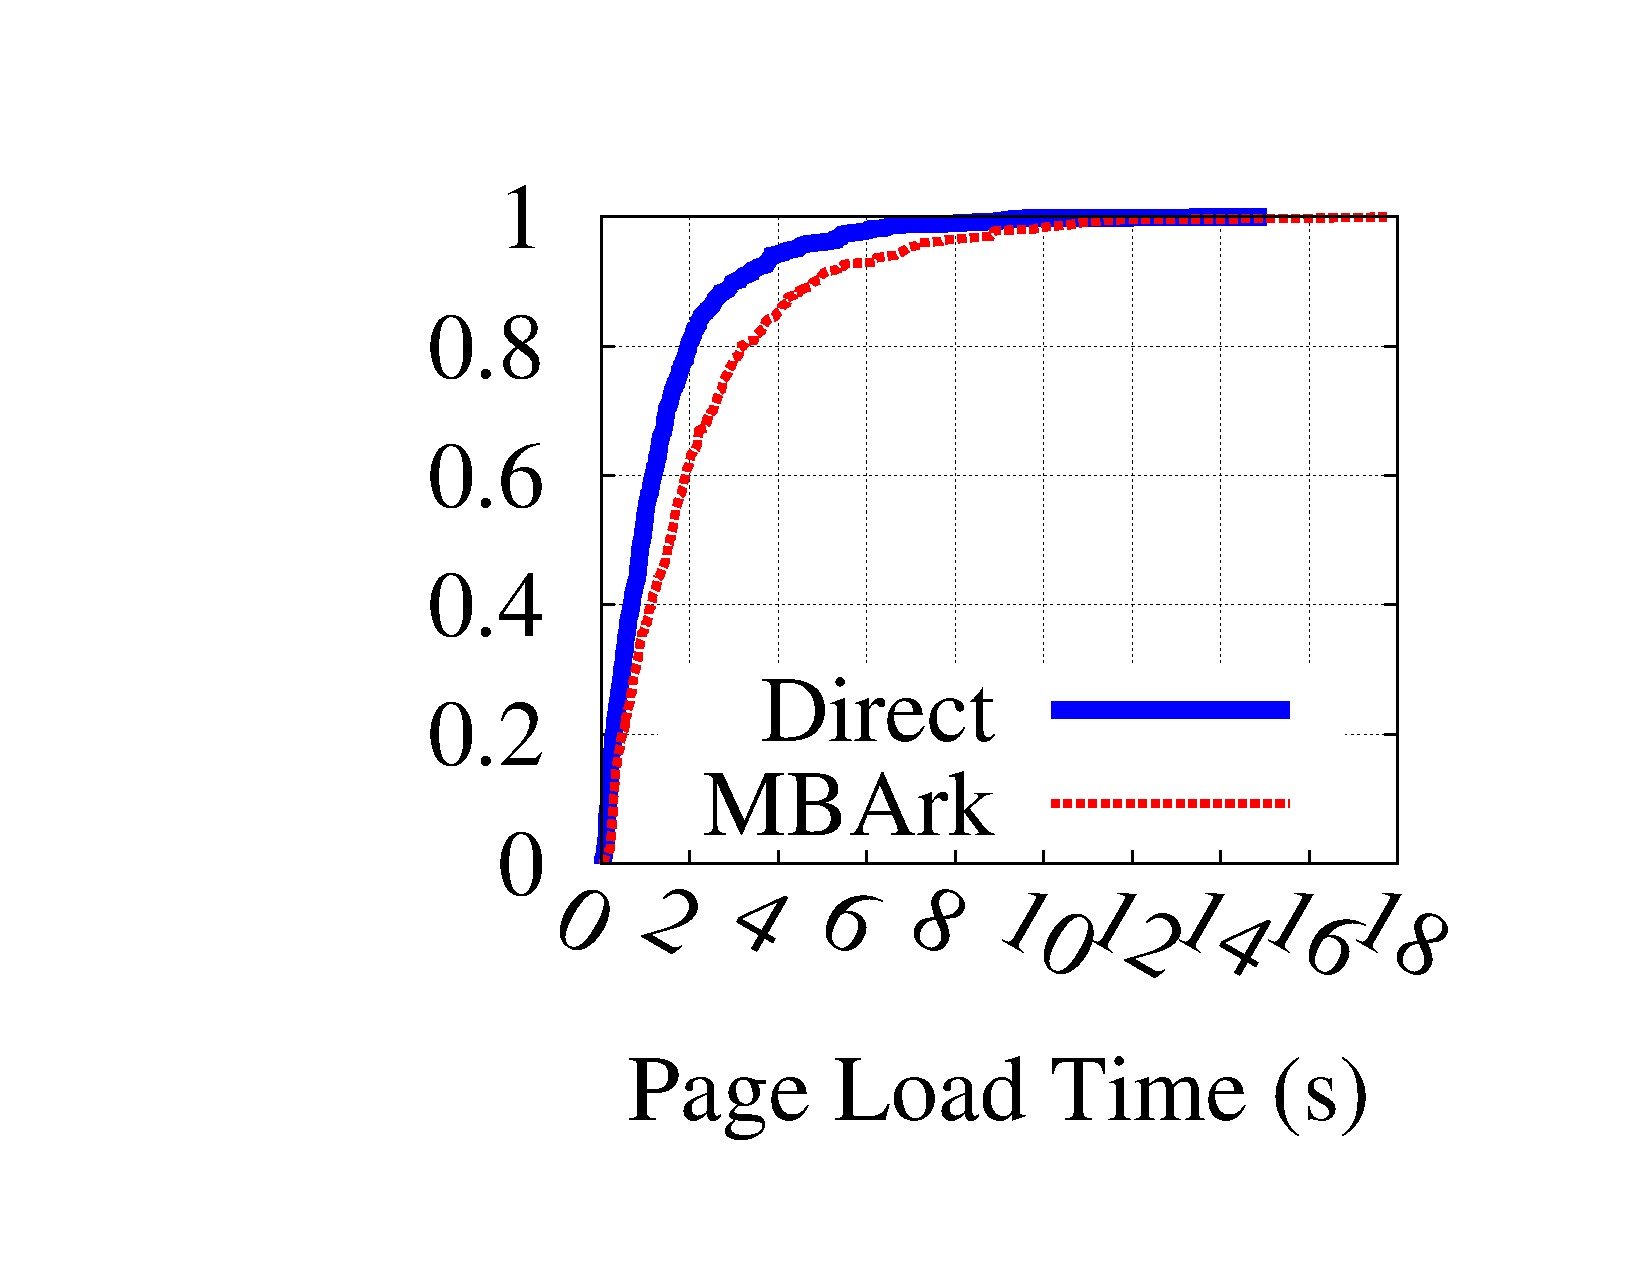
\includegraphics[height=1in]{fig/e2e_loadtimes}
  &\hspace{-10pt}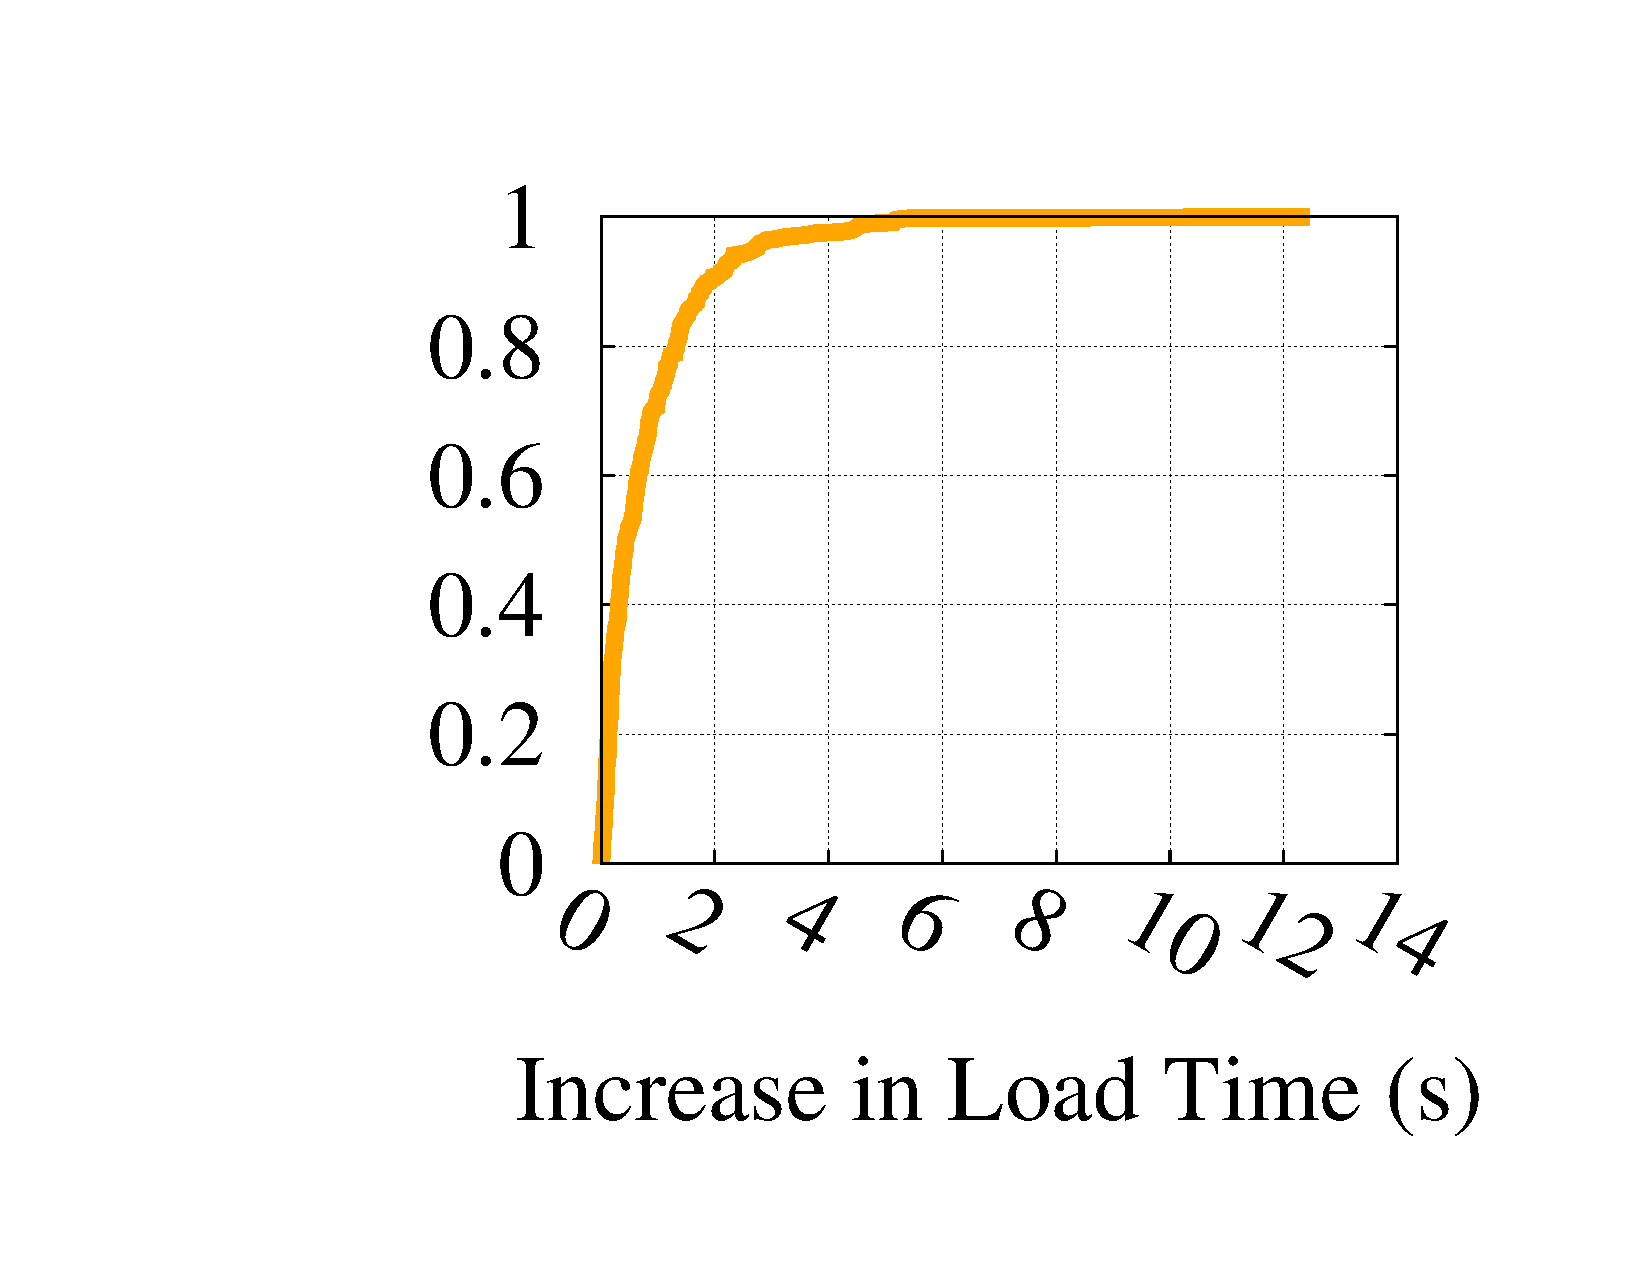
\includegraphics[height=1in]{fig/e2e_delta_absolute}
  &\hspace{-10pt}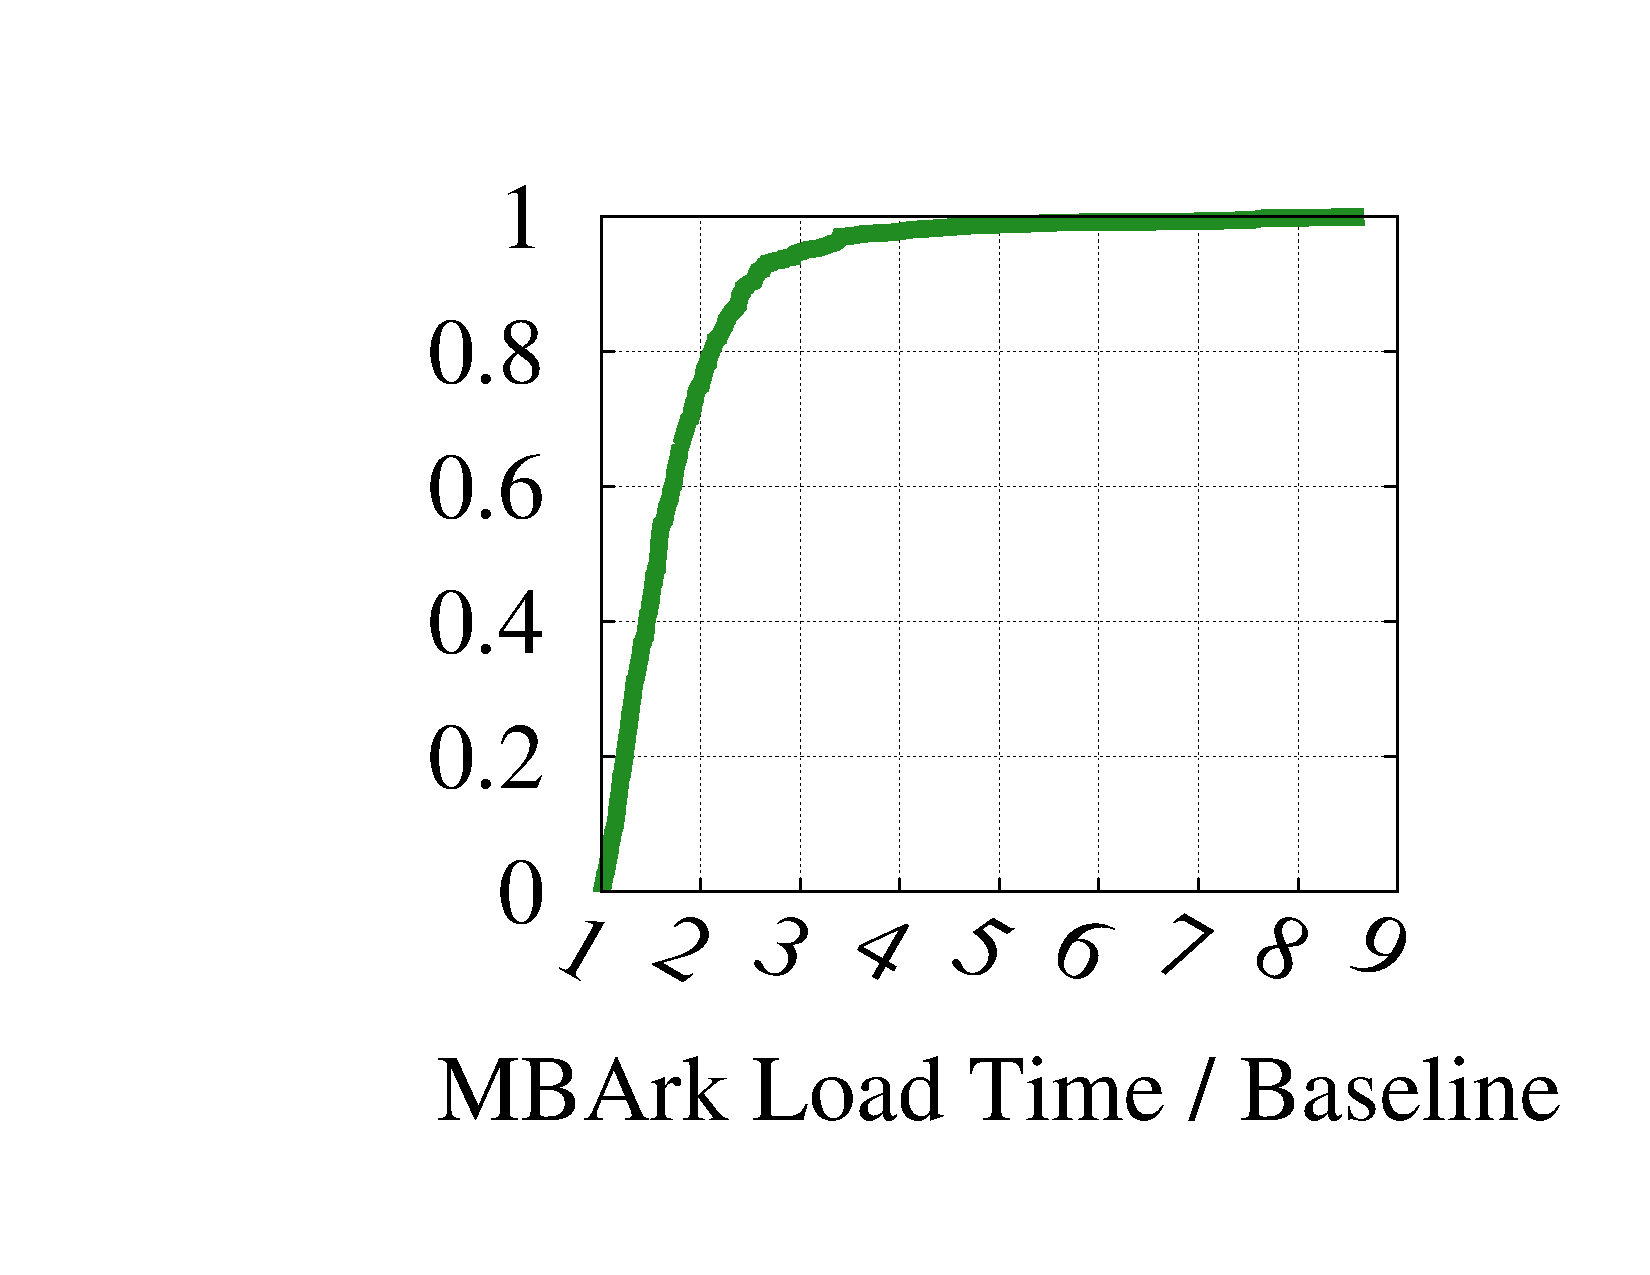
\includegraphics[height=1in]{fig/e2e_delta_relative}
  \\
  &(a)&(b)&(c)\\
  \end{tabular}
  \vspace{-10pt}
  \caption[]{\label{fig:e2eloads} Page load times through \sys compared to direct download.}
  \vspace{-10pt}
\end{figure}
{\it What overheads does \sys impose on web download times?}
\todo{CL}

{\it How much does bandwidth increase between the gateway and the cloud from using \sys? How much would this bandwidth increase an enterprises networking costs?}
\sys sends all network traffic to and from the middlebox service provider for processing, before sending that traffic out to the Internet at large. In NFV contexts, the clients' middlebox service provider and network connectivity provider are one and the same and one might expect costs for relaying the traffic to and from the middleboxes to be rolled in to one `package.' 
However, in the APLOMB setting, the middlebox service provider is a cloud, meaning that the client must pay a third party ISP to transfer the data to and from the cloud, before paying that ISP a third time actually transfer the data over the network.

Beyond sending the primary traffic 3 times (2$\times$ on the uplink, $1\times$ on the downlink), the gateway also inflates the size of this traffic due to encryption overhead:
\begin{itemize}
  \item If the enterprise uses IPv4, there is a 20-byte per-packet cost to convert from IPv4 to IPv6. If the enterprise uses IPv6 by default, there is no such cost.
  \item If HTTP proxying is enabled, there are on average 132 bytes per request in additional encrypted data.
  \item If HTTP IDS is enabled, there is at worst a 5$\times$ overhead on all HTTP payloads.
\end{itemize}
We used te m57 trace to understand how these overheads would play out in aggregate for an enterprise.
On the uplink, from the gateway to the middlebox service provider, traffic would increase by 2.5\% due to encryption costs for a Header-Only Gateway. Traffic would increase by 4.3$\times$ on the uplink for a bytestream-aware gateway. 

Using current bandwidth pricing~\cite{comcast-costs, megapath-costs, verizon-costs}, we can observe how such inflation would increase costs: 
\todo{Getting frustrated with these numbers so leaving them here and will come back to them. Megapath offers a dedicated link at 5x5Mbps for \$250/mo; 20x20Mbps for \$1300/mo. Comcast offers enterprise cable at 150/20Mbps for \$250/mo. The three way bounce should result in a cost increase of 15-50\%, depending on how much the internal link is providioned for. The DPI should be 2-3 times that, so, between 30-150\%... 
}

\subsection{Header-Only \sys}
We first evaluate Header-only \sys, with its stateless gateway. 
Header-only \sys supports all middleboxes which operate only on IP and TCP headers (\eg{}, firewalls, NATs, and L4 Load Balancers) , as well as proxies for non-pipelined HTTP connections (as discussed in \S\ref{sec:proxy}).
The primary cost at the gateway comes from implementing the range encryption algorithm we developed in~\ref{sec:rangematch}. 
Unlike existing order preserving algorithms~\cite{mope,BCLO} which require on the order of milliseconds for every encryption operation, range encryption can keep up with packet processing workloads, requiring only 3$\mu$s per packet to encrypt (three orders of magnitude faster than previous approaches).
We discuss the range match scheme and the gateway in the following subsection, after which we present the performance of individual middleboxes when modified for \sys.

\subsubsection{Header-Only Gateway}
\begin{figure}[t]
  \centering
  \begin{tabular}{cc}
  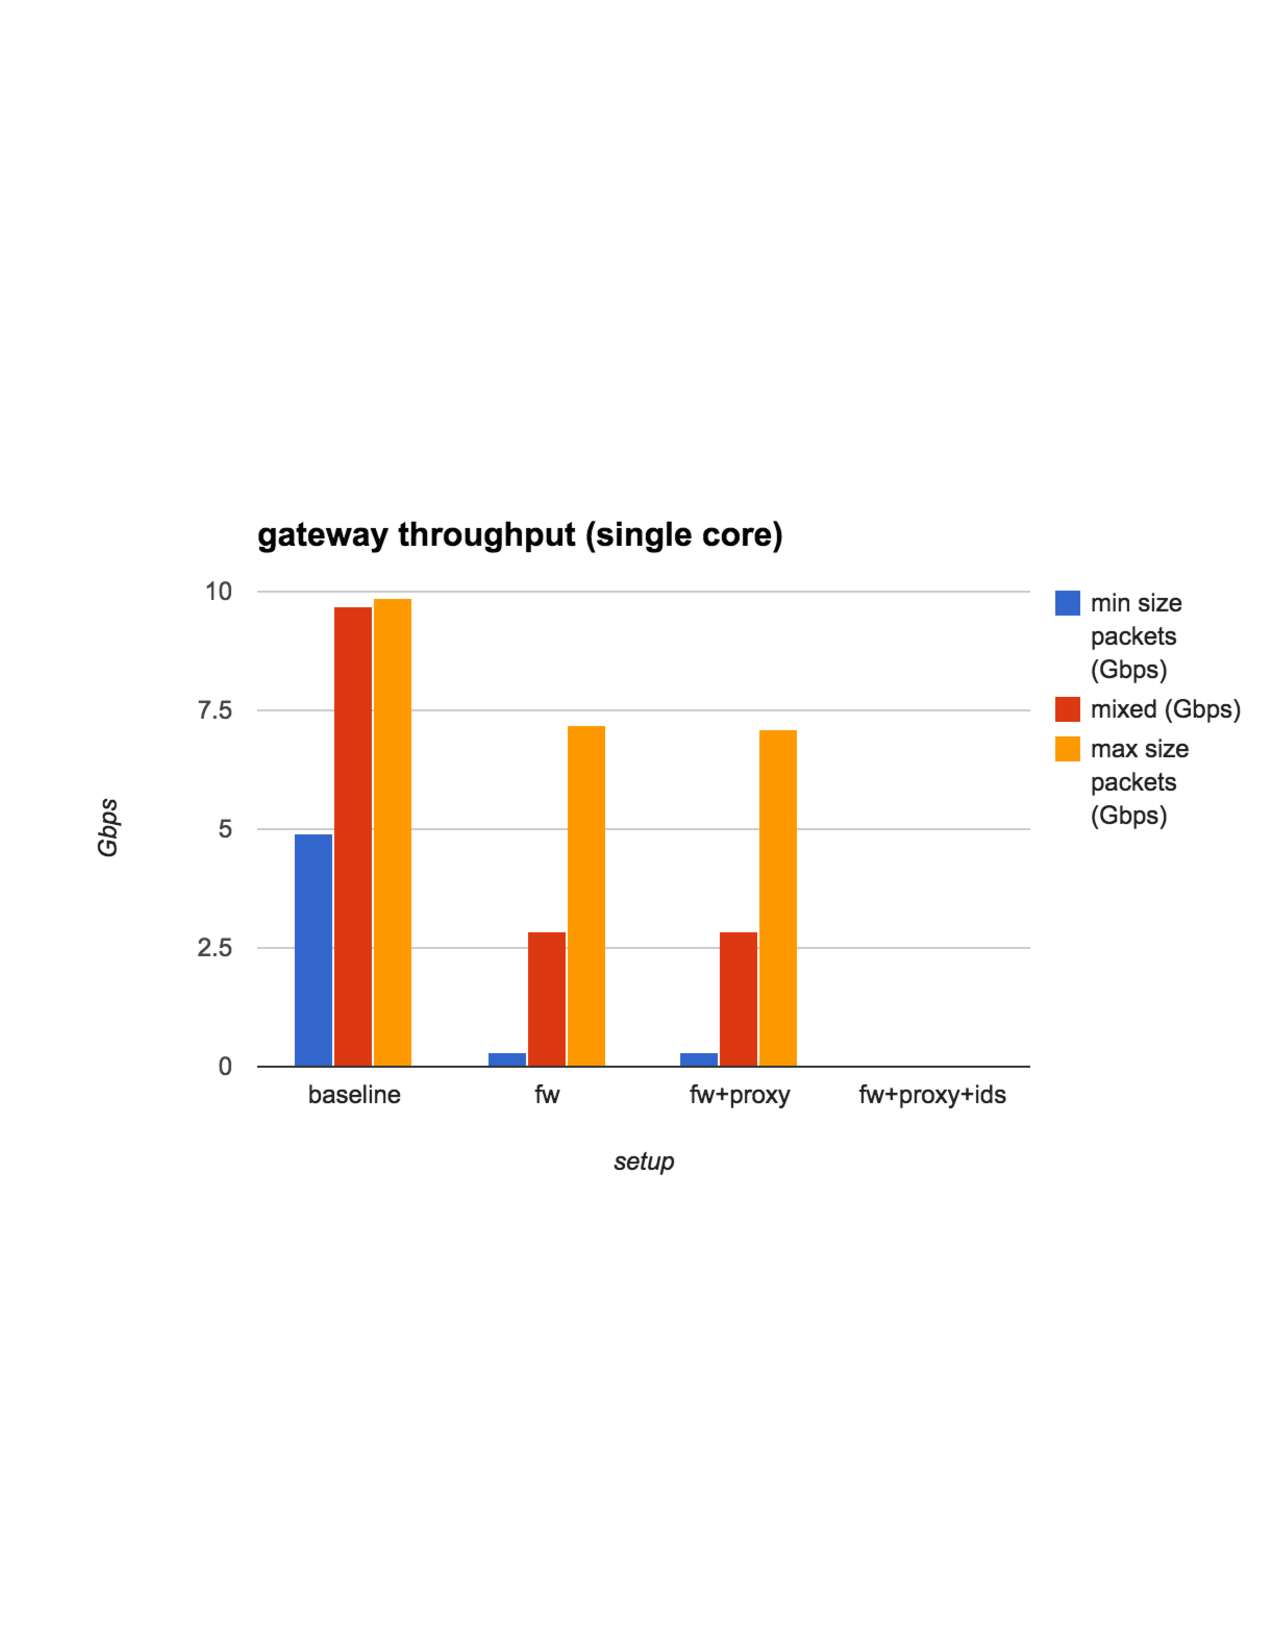
\includegraphics[height=1.25in]{fig/gatewayxput}&
  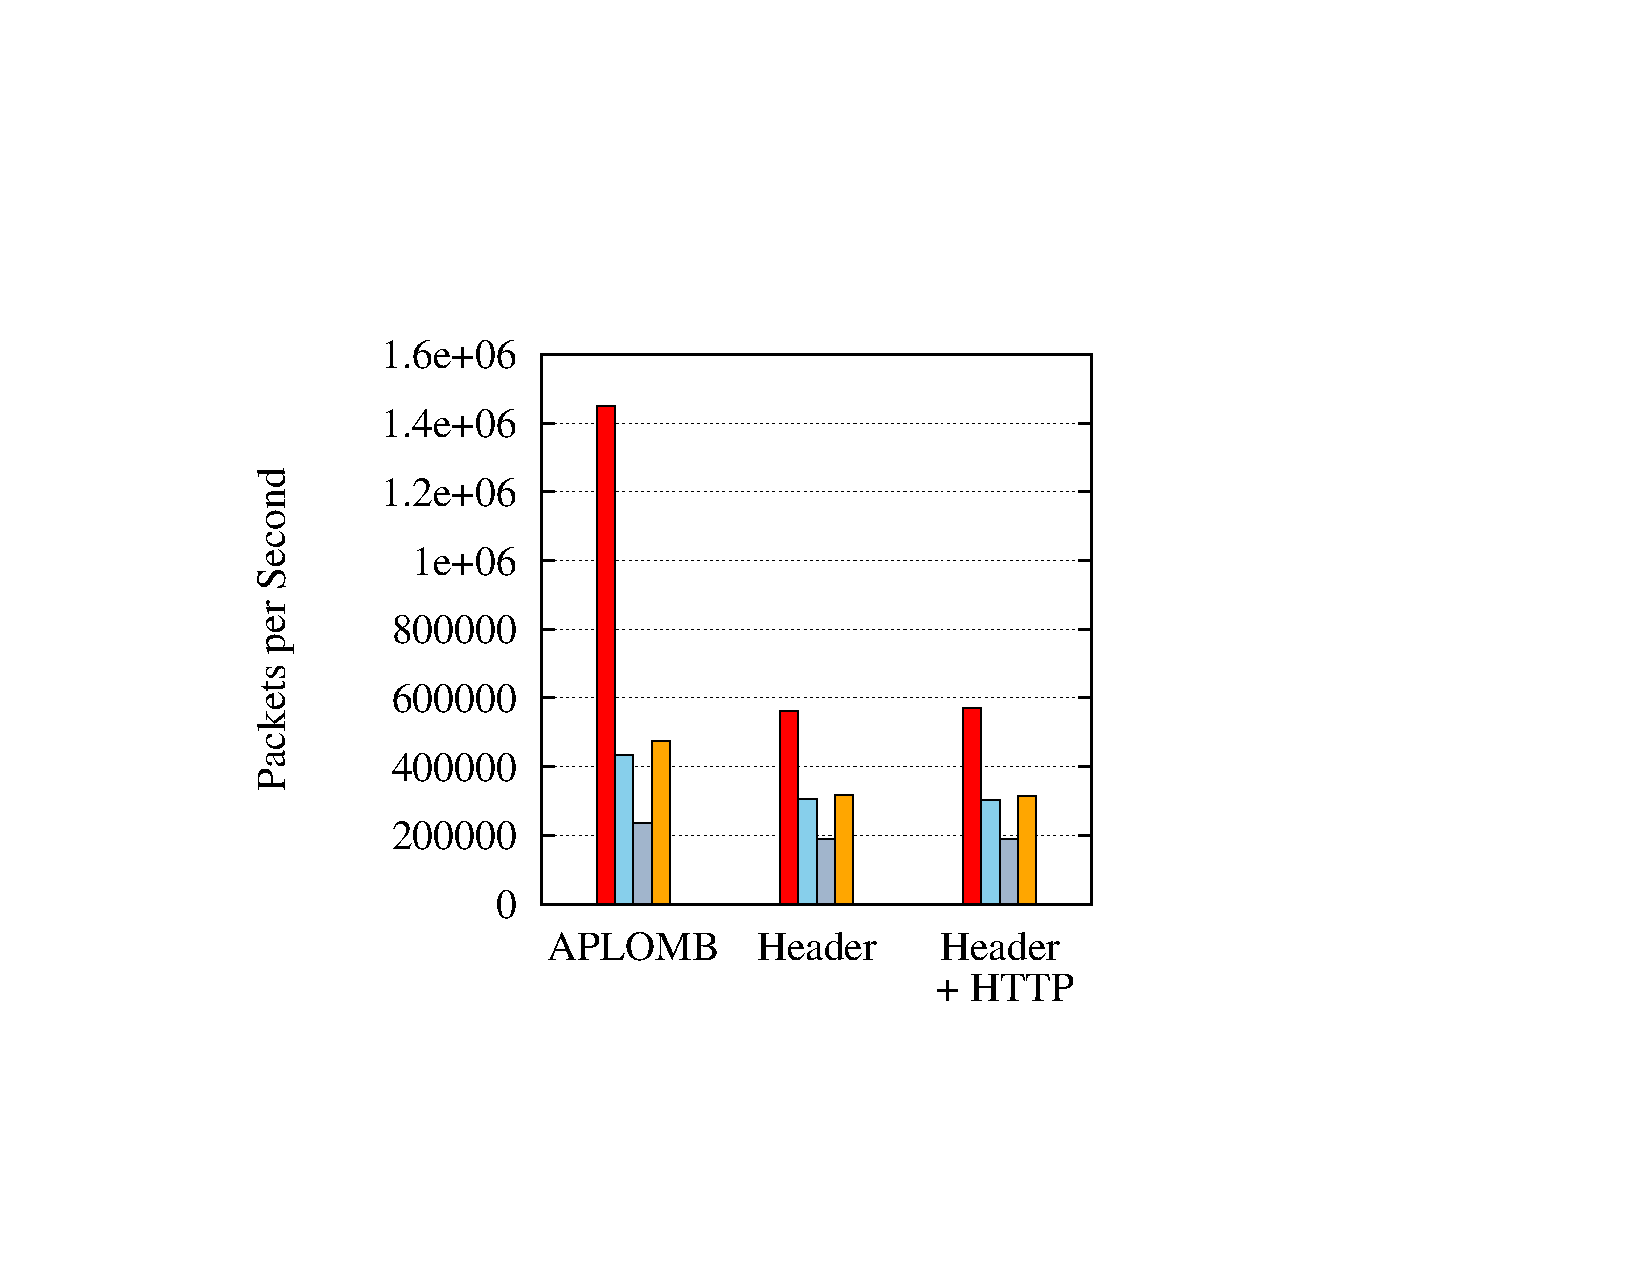
\includegraphics[height=1.25in]{fig/gateway_pps}\\
  \end{tabular}
  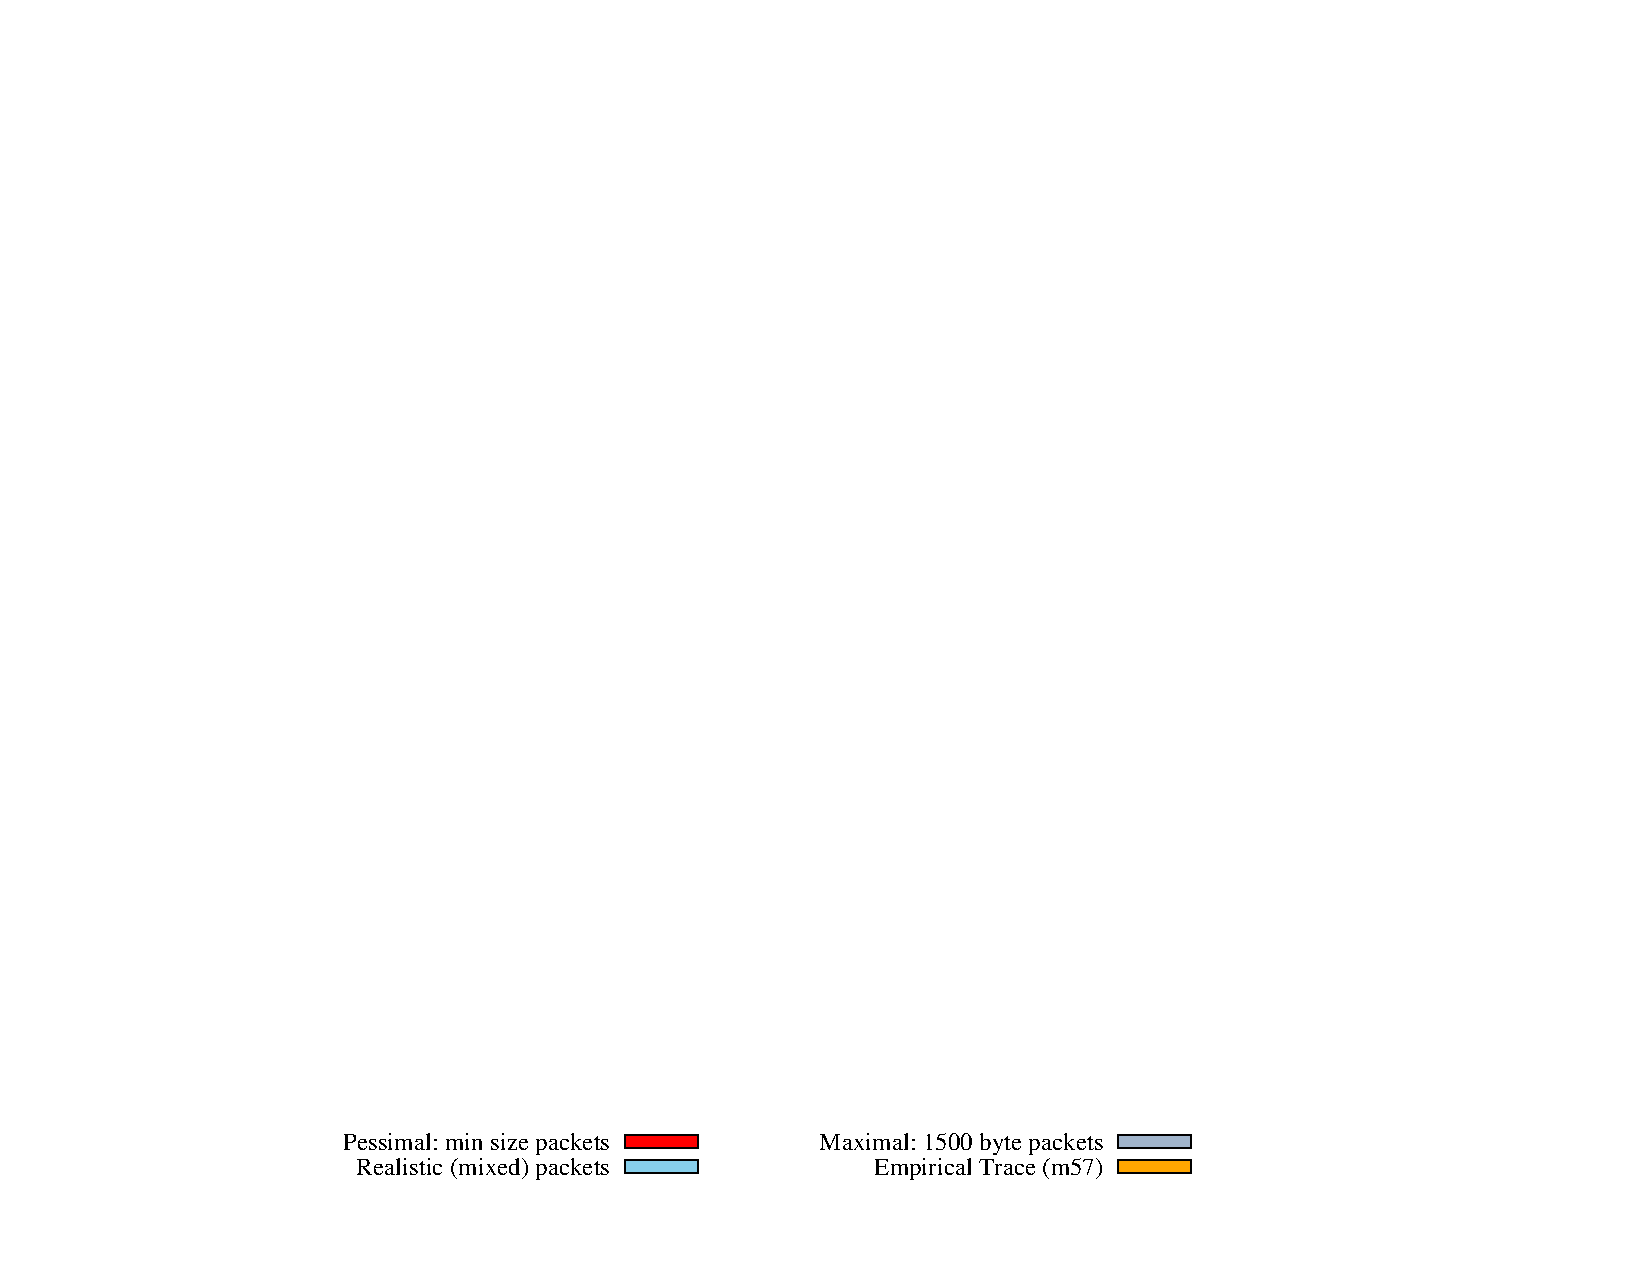
\includegraphics[width=2.75in]{fig/key}
  \vspace{-10pt}
  \caption[]{\label{fig:gwxput} Throughput/Packets per Second on a single core at the statless gateway.}
  \vspace{-10pt}
\end{figure}

\noindent{\it How does encryption impact throughput at the outsourcing gateway?}
Figure~\ref{fig:gwxput} shows the gateway throughput when encrypting traffic to send to the cloud, first with normal redirection (as used in APLOMB~\cite{aplomb}), then with \sys's IP/TCP-header encryption, and finally with IP/TCP-header encryption as well as HTTP/proxy encryption. There is little difference between the HTTP overhead and the IP/TCP overhead, as the HTTP encryption only occurs on HTTP requests -- a small fraction of packets. Overall, MBArk encryption for the stateless gateway reduces by about 60\% relative to baseline APLOMB encryption in the worst case (the min-sized workload; the reduction for the empirical (m57) workload is 38\%. Hence, an enterprise moving from a traditional outsourcing approach to MBark would need to provision at worst around 2.5$\times$ the number of processors at the outsourcing gateway.

\begin{figure}[t]
  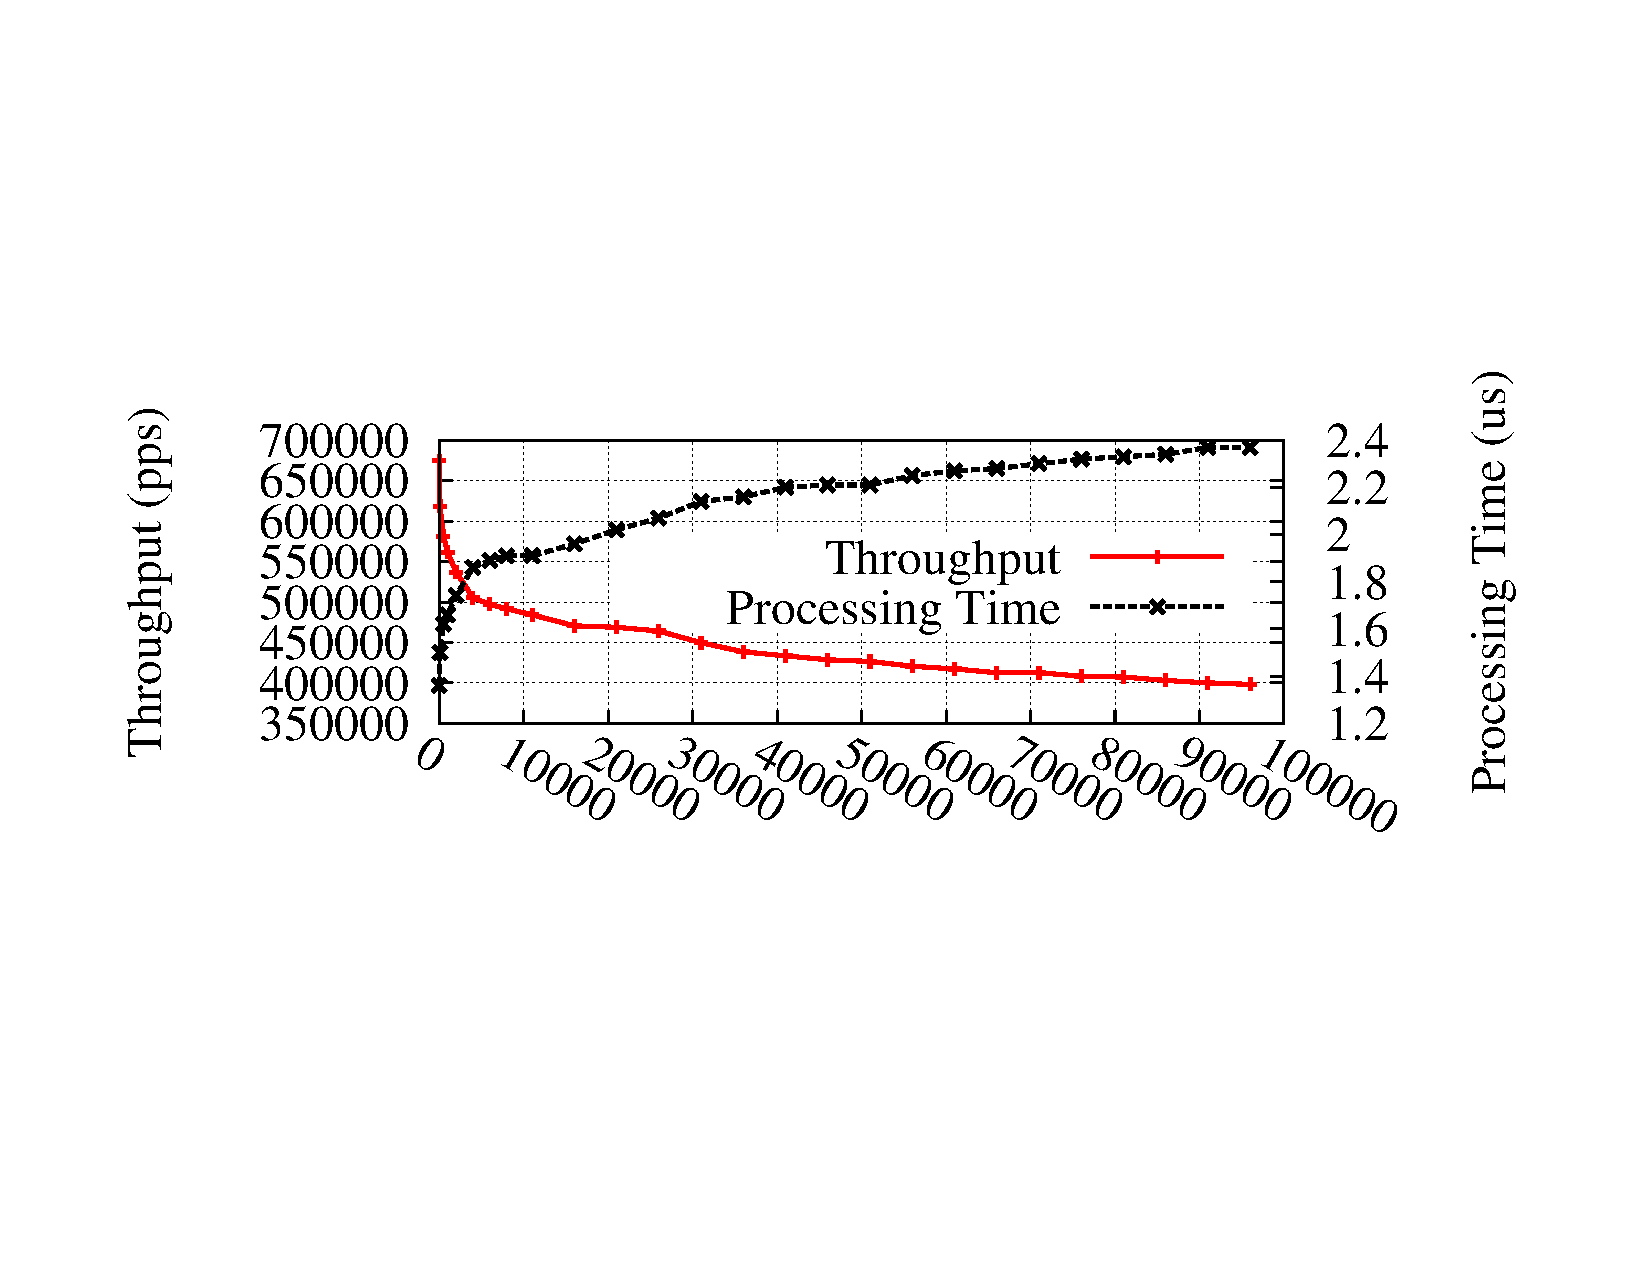
\includegraphics[width=3.25in]{fig/xputrange}
  \vspace{-10pt}
  \caption[]{\label{fig:xputrange} Throughput as number of rules for range encrypt increases.}
  \vspace{-10pt}
\end{figure}

\noindent{\it How do throughput and latency at the gateway scale with the number of rules for range encryption?} 
In \S\ref{sec:range}, we discussed how our range encryption scheme stores encrypted values in a tree; every packet encryption requires a traversal of this tree.
Hence, as the size of the tree goes larger, we can expect to require more time to process each packet and throughput to decrease.
We measure this effect in Figure~\ref{fig:xputrange}. 
On the $y_1$ axis, we show the aggregate per packet throughput at the gateway as the number of rules from 0 to 100k. The penalty here is logarithmic, which is the expected performance of tree data structures. From 0-10k rules, throughput drops from 670Kpps to 480Kpps; after this point the performance penalty of additional rules tapers off. Adding an aditional 90k rules drops throughput to 400Kpps.
On the $y_2$ axis, we measure the processing time per packet, \ie{}, the amount of time from when the gateway begins encrypting the packet to when the gateway completes encrypting the packet; the processing time follows the same logarithmic trend.
\todo{new latency numbers}

\noindent{\it Is range encryption faster than existing order preserving algorithms?}
Our range encryption is the only encryption scheme that has low enough latency for packet processing while preserving the ordering information needed for firewall rules. 
Existing order-preserving approaches require multiple round trip times -- and hence many milliseconds -- for each encryption operation.
Our range encoding approach encrypts each value in microseconds.
We compare against mOPE~\cite{mope} and BCLO~\cite{BCLO} below:

\begin{table}[h]
\centering
\begin{tabular}{c|c|c|c}
Operation&BCLO~\cite{BCLO}&mOPE~\cite{mope}&\sys\\
\hline
\hline
Encrypt, 10K rules&9333$\mu$s&6640$\mu$s&1,95$\mu$s\\
\hline
Encrypt, 100K rules&9333$\mu$s&8300$\mu$s&3$\mu$s\\
\hline
Decrypt&169$\mu$s&0.128$\mu$s&0.128$\mu$s\\
\hline
\end{tabular}
\end{table}

\noindent{\it What is the memory overhead of the stateful range map encryption scheme?}
Storing 10k rules in memory requires 1.6MB, and storing 100k rules in memory requires 28.5MB -- using unoptimized C++ objects.
This state overhead is negligible on any modern server.

\subsubsection{Header-Only Middleboxes}

\begin{table}[t!]
\begin{tabular}{p{3cm}|p{2cm}|p{2cm}}
Application &  Baseline Throughput & \sys Throughput \\
\hline \hline
IP Firewall &     &  \\
Application Firewall  & & \\
NAT &   &   \\
IP Forwarding  & & \\
%VPN Gateway &  &  &  \\ 
Load Balancer L4  & & \\
%Load Balancer L7 & & & \\
%WAN optimizer  & & & \\
Web Proxy & &\\
%IDS & & & \\
%Exfiltration/parental filtering & & &  \\
\end{tabular}
\caption{Middlebox applications supported by Header-Only \sys; throughput measured with an emprical traffic workload. \label{tbl:appsxput}}
\vspace{-10pt}
\end{table}

\noindent{\it Is throughput reduced at the middleboxes due to Header-Only \sys?}
Table~\ref{tbl:appsxput}...\todo{FILL IN}



\noindent{\bf Firewalls.} 
{\it Does \sys support all rules in a typical firewall configuration? How much does the ruleset ``expand'' due to encryption?}

\noindent{\it How often do updates to the firewall require a rule refresh? How long does it take to refresh rules at the firewall?}

\noindent{\bf NAT.}
\noindent{\bf LB...}

\noindent{\bf Proxy/Caching.}
{\it How many active connections per second can the Proxy accept? How does this compare to an unencrypted Proxy implementation, like Squid?}

{\it What improvement in page load times does a client experience due to proxying, relative to no proxy at all? Relative to an unencrypted proxy implementation?}



\subsection{\sys with Bytestream Reconstruction}
In \S\ref{sec:something}, we discussed how the \sys gateway must be stateful to support bytestream-aware applications in order to encrypt end-to-end payloads properly for intrusion detection, and in order to parse the HTTP header for proxying pipelined HTTP connections. 
In Figure~\ref{fig:dpigateway}, we compare the stateful, bytestream-aware gateway throughput to the stateless gateway throughput. 
The overhead introduced by the bytestream-aware gateway is twofold: (1) the cost of statefull connection-keeping, and (2) the increased encryption cost, as cryptographic operations are performed over the payload (as much as 1500 bytes) rather than the headers (<30 bytes).
We observe that~\todo{JS.}

We now evaluate the performance of our two bytestream-aware middleboxes: a proxy for pipelined connections, and an IDS.

\noindent{\bf Intrusion Detection}
Our IDS is based on BlindBox~\cite{blindbox}. However, \sys affords better performance and stronger privacy than BlindBox. BlindBox incurs a substantial `setup cost' every time a client initiates a new connection. With \sys, however, the gateway and the cloud maintain one, long-term persistent connection. 
Hence, this setup cost is paid once when the gateway is initially configured. This results in two benefits:

\noindent{\it (1) End-to-end performance improves.} Where BlindBox incurs an initial handshake of 414s~\cite{blindbox} to open a new connection, clients under MBark never pay this cost; instead they perform a normal TCP or SSL handshake of only 3-5 RTTs. In our testbed, this amounts to betweeh 30 and 100 ms, depending on the site and protocol -- an improvement of 4 orders of magnitude.

\noindent{\it (2) Security improves.} As we presented in \S\ref{sec:ids}, BlindBox operates at one of two security levels: a stronger security level for exact-match strings, and a weaker security level for regular expressions. The stronger security level requires a round of handshake for each rule, but the weaker security level does not require more handshakes for each regular expression. 
With \sys, the initial handshake/setup is performed exactly once, between the gateway and the middlebox. 
Hence, we can convert regular expressions to exact match strings, even if they result in many hundreds of times more exact match rules. 
Consequently, more rules can be detected using the stronger security guarantee, without incurring any handshake overhead.
Using IDS rulesets from Snort, we converted regular expressions to exact match strings as discussed in \S\ref{sec:ids}; we were able to convert about half of all regular expressions to a finite number of exact match strings. 
Consequently, \sys can detect more then 80-88\% of attacks using the higher security level, rather than 42-67\% as with BlindBox:

\begin{table}[h]
  \centering
  \begin{tabular}{l|c|c}
    {\bf Dataset}&{\bf Exact Match}&{\bf Prob. Cause}\\
    \hline
    \hline
    BB: Community&67\%&100\%\\
    \hline
    \sys: Community&88.7\%&100\%\\

    \hline
    \hline
    BB: Emerging Threats&42\%&100\%\\
    \hline
    \sys: Emerging Threats&79.8\%&100\%\\
    \hline
  \end{tabular}
\end{table}

\noindent{\bf Proxy.} \todo{Can we say something here so it doesn't sound like we have a special gateway just for IDS? Because we do need this for IDS -- maybe, how much improvement over the non-pipeline proxy do we get?}

